%% Copernicus Publications Manuscript Preparation Template for LaTeX Submissions
%% ---------------------------------
%% This template should be used for copernicus.cls
%% The class file and some style files are bundled in the Copernicus Latex Package, which can be downloaded from the different journal webpages.
%% For further assistance please contact Copernicus Publications at: production@copernicus.org
%% https://publications.copernicus.org/for_authors/manuscript_preparation.html


%% Please use the following documentclass and journal abbreviations for preprints and final revised papers.

%% 2-column papers and preprints
\documentclass[npg, manuscript]{copernicus}



%% Journal abbreviations (please use the same for preprints and final revised papers)


% Advances in Geosciences (adgeo)
% Advances in Radio Science (ars)
% Advances in Science and Research (asr)
% Advances in Statistical Climatology, Meteorology and Oceanography (ascmo)
% Annales Geophysicae (angeo)
% Archives Animal Breeding (aab)
% Atmospheric Chemistry and Physics (acp)
% Atmospheric Measurement Techniques (amt)
% Biogeosciences (bg)
% Climate of the Past (cp)
% DEUQUA Special Publications (deuquasp)
% Drinking Water Engineering and Science (dwes)
% Earth Surface Dynamics (esurf)
% Earth System Dynamics (esd)
% Earth System Science Data (essd)
% E&G Quaternary Science Journal (egqsj)
% European Journal of Mineralogy (ejm)
% Fossil Record (fr)
% Geochronology (gchron)
% Geographica Helvetica (gh)
% Geoscience Communication (gc)
% Geoscientific Instrumentation, Methods and Data Systems (gi)
% Geoscientific Model Development (gmd)
% History of Geo- and Space Sciences (hgss)
% Hydrology and Earth System Sciences (hess)
% Journal of Bone and Joint Infection (jbji)
% Journal of Micropalaeontology (jm)
% Journal of Sensors and Sensor Systems (jsss)
% Magnetic Resonance (mr)
% Mechanical Sciences (ms)
% Natural Hazards and Earth System Sciences (nhess)
% Nonlinear Processes in Geophysics (npg)
% Ocean Science (os)
% Polarforschung - Journal of the German Society for Polar Research (polf)
% Primate Biology (pb)
% Proceedings of the International Association of Hydrological Sciences (piahs)
% Safety of Nuclear Waste Disposal (sand)
% Scientific Drilling (sd)
% SOIL (soil)
% Solid Earth (se)
% The Cryosphere (tc)
% Weather and Climate Dynamics (wcd)
% Web Ecology (we)
% Wind Energy Science (wes)


%% \usepackage commands included in the copernicus.cls:
%\usepackage[german, english]{babel}
%\usepackage{tabularx}
%\usepackage{cancel}
%\usepackage{multirow}
%\usepackage{supertabular}
%\usepackage{algorithmic}
%\usepackage{algorithm}
%\usepackage{amsthm}
%\usepackage{float}
%\usepackage{subfig}
%\usepackage{rotating}

%\newcommand{\nb}{\textsuperscript{\color{blue}{#1}}}

\begin{document}

\title{On the guess consistency in multi-incremental multi-resolution variational data assimilation}


% \Author[affil]{given_name}{surname}

\Author[1]{Nicolas}{Baillot d'Étiaux}
\Author[2]{Benjamin}{Ménétrier}
\Author[3]{Selime}{Gürol}
\Author[4]{Yann}{Michel}

\affil[1]{CNRM, Université de Toulouse, Météo-France, CNRS, Toulouse, France}
\affil[2]{IRIT, ...}
\affil[2]{CERFACS, ...}
\affil[4]{Météo-France, ...}

%% The [] brackets identify the author with the corresponding affiliation. 1, 2, 3, etc. should be inserted.

%% If an author is deceased, please mark the respective author name(s) with a dagger, e.g. "\Author[2,$\dag$]{Anton}{Smith}", and add a further "\affil[$\dag$]{deceased, 1 July 2019}".

%% If authors contributed equally, please mark the respective author names with an asterisk, e.g. "\Author[2,*]{Anton}{Smith}" and "\Author[3,*]{Bradley}{Miller}" and add a further affiliation: "\affil[*]{These authors contributed equally to this work.}".


\correspondence{Benjamin Ménétrier (benjamin.menetrier@irit.fr)}

\runningtitle{TEXT}

\runningauthor{TEXT}





\received{}
\pubdiscuss{} %% only important for two-stage journals
\revised{}
\accepted{}
\published{}

%% These dates will be inserted by Copernicus Publications during the typesetting process.


\firstpage{1}

\maketitle



\begin{abstract}
Variational Data Assimilation (DA) schemes are often used to adress high dimensional non-linear problems in operational applications in the Numerical Wheather Prediction (NWP) domain. Because of the high computational cost of such minimization problems, various methods can be applied to improve the convergence at a reasonable numerical cost. One of these methods currently applied in operational DA schemes is the multi-incremental approach that consists in solving a succession of linearized versions of the original non-linear problem in several outer loops, by using well known algorithms to ensure the convergence of the linear problem at the inner loop level, and using the solution of the inner loops to update the problem at each outer loop. In order to save computational cost, the multi-incremental multi-resolution method consists in starting the minimization at a lower resolution than the original one, and increasing it at the outer loop level until the full resolution of the problem. In such a scheme, the way to compute the new guess at each outer loop from the previous iterations is crucial. We adress the question of the guess consistency in the standard method currently used in operational systems, and also present a new method which ensures the guess consistency and need simpler calculations. 
On the other hand, the conditionning of NWP problems is often poor, and one can use preconditionning techniques in order to improve the convergence. We have applied the multi-incremental multi-resolution scheme to a simplified problem in order to study the guess consistency as well as the equivalence between two well known preconditionnings ("full" $\mathbf{B}$ or "square root" $\mathbf{B}$) in such a scheme. Some equivalence conditions between the updating methods and the two preconditionnings are drawn according to the way the resolution change is realised at the outer loop level.
\end{abstract}


%\copyrightstatement{TEXT} %% This section is optional and can be used for copyright transfers.


%---------------------------------------------------------------------------------
\introduction
intro...

%---------------------------------------------------------------------------------
\section{Data Assimilation Problem}
% Introducing the global problem.
In Data Assimilation (DA), one wants to minimize the following non linear cost function representing the ability of a model state to be compatible with observations:
\begin{align}
\hspace{-0.7cm} \mathcal{J}(\mathbf{x}) = \frac{1}{2} \left(\mathbf{x}-\mathbf{x}^b\right)^\mathrm{T} \mathbf{B}^{-1} \left(\mathbf{x}-\mathbf{x}^b\right) + \frac{1}{2} \left(\mathbf{y}^o-\mathcal{H}(\mathbf{x})\right)^\mathrm{T} \mathbf{R}^{-1} \left(\mathbf{y}^o-\mathcal{H}(\mathbf{x})\right),
\end{align}
where $\mathbf{x} \in \mathbb{R}^n$ is the state in model space of size $n$, $\mathbf{x}^b \in \mathbb{R}^n$ is the background state, $\mathbf{B} \in \mathbb{R}^{n \times n}$ is the background error covariance matrix, $\mathbf{y}^o \in \mathbb{R}^p$ is the observation vector  in observation space of size $p$ (note that in general $p<n$), $\mathbf{R} \in \mathbb{R}^{p \times p}$ is the observation error covariance matrix, and $\mathcal{H} : \mathbb{R}^n \rightarrow \mathbb{R}^p$ is the observation operator which maps the model space to the observation space. 

\subsection{Problem linearization}
In general the observation operator is nonlinear and can be linearized around a guess state $\mathbf{x}^g_k \in \mathbb{R}^n$ so that: 
\begin{align}
 \mathcal{H}(\mathbf{x}) \approx \mathcal{H}(\mathbf{x}^g_k) + \mathbf{H}_k \delta \mathbf{x}_k \quad \textrm{for}\ \mathbf{x} \approx \mathbf{x}^g_k,
\end{align}
defining the increment $\delta \mathbf{x}_k =  \mathbf{x}-\mathbf{x}^g_k$, and where $\mathbf{H}_k \in \mathbb{R}^{p \times m}$ is the observation operator linearized around the guess state: 
\begin{align}
 \mathbf{H}_{k,ij} = \left.\frac{\partial \mathcal{H}_i}{\partial x_j}\right|_{\mathbf{x} = \mathbf{x}^g_k}.
\end{align}
Instead of minimizing the full cost function $\mathcal{J}(\mathbf{x})$, it is now possible to minimize successive quadratic approximations around successive guess states:
\begin{align}
\label{eq:cost_quad}
J \left(\delta \mathbf{x}_k\right) = \frac{1}{2} \left(\delta \mathbf{x}_k-\delta \mathbf{x}^b_k\right)^\mathrm{T} \mathbf{B}^{-1} \left(\delta \mathbf{x}_k-\delta \mathbf{x}^b_k\right) + \frac{1}{2} \left(\mathbf{d}_k - \mathbf{H}_k \delta \mathbf{x}_k\right)^\mathrm{T} \mathbf{R}^{-1} \left(\mathbf{d}_k - \mathbf{H}_k \delta \mathbf{x}_k\right)
\end{align}
where $k$ indicates the $k^{th}$ iteration (hereafter these iterations are called "outer loops" since the minimization of the successive approximations are realized using well known iterative solvers such as Lanczos alorithms. We call "inner loops" the iterations of these algorithms), $\delta \mathbf{x}^b_k = \mathbf{x}^b - \mathbf{x}^g_k$ is the background increment and $\mathbf{d}_k = \mathbf{y}^o - \mathcal{H}(\mathbf{x}^g_k)$ is the innovation vector.\\

Setting the gradient of $J(\delta \mathbf{x}_k)$ to zero gives the analysis increment $\delta \mathbf{x}^a_k$:
\begin{align}
\label{eq:inc}
& \ \mathbf{B}^{-1} \left(\delta \mathbf{x}^a_k - \delta \mathbf{x}^b_k\right) - \mathbf{H}_k^\mathrm{T} \mathbf{R}^{-1} \left(\mathbf{d}_k - \mathbf{H}_k \delta \mathbf{x}^a_k\right) = 0 \nonumber \\
\Leftrightarrow & \ \left(\mathbf{B}^{-1} + \mathbf{H}_k^\mathrm{T} \mathbf{R}^{-1} \mathbf{H}_k\right) \delta \mathbf{x}^a_k = \mathbf{B}^{-1} \delta \mathbf{x}^b_k + \mathbf{H}_k^\mathrm{T} \mathbf{R}^{-1} \mathbf{d}_k \nonumber \\
\Leftrightarrow & \ \boxed{\mathbf{A}^\mathbf{x}_k \delta \mathbf{x}^a_k = \mathbf{b}^\mathbf{x}_k}
\end{align}
where $\mathbf{A}^\mathbf{x}_k \in \mathbb{R}^{n \times n}$ and the right hand side $\mathbf{b}^\mathbf{x}_k \in \mathbb{R}^{n}$ are defined as:
\begin{align}
\mathbf{A}^\mathbf{x}_k & = \mathbf{B}^{-1} + \mathbf{H}_k^\mathrm{T} \mathbf{R}^{-1} \mathbf{H}_k , \\
\mathbf{b}^\mathbf{x}_k & = \mathbf{B}^{-1} \delta \mathbf{x}^b_k + \mathbf{H}_k^\mathrm{T} \mathbf{R}^{-1} \mathbf{d}_k .
\end{align}
The problem can now be solved in this form using Gauss-Newton algorithm. It is very common to use the background state as a guess for the first iteration $k=1$: $\mathbf{x}^g_1 = \mathbf{x}^b$. Then for $k>1$, the analysis of the previous iteration is used to define the guess: $\mathbf{x}^g_k = \mathbf{x}^a_{k-1}$. Thus, the first background increment is $\delta \mathbf{x}^b_1 = \mathbf{x}^g_1 - \mathbf{x}^b = 0$, and the following ones can be computed as:
\begin{align}
\delta \mathbf{x}^b_k & = \mathbf{x}^b - \mathbf{x}^g_k, \nonumber \\
& = \mathbf{x}^b - \mathbf{x}^a_{k-1}, \nonumber \\
& = \mathbf{x}^b - \left(\mathbf{x}^g_{k-1} + \delta \mathbf{x}^a_{k-1}\right), \nonumber \\
& = \delta \mathbf{x}^b_{k-1} - \delta \mathbf{x}^a_{k-1},
\end{align}
which can be combined recursively to yield:
\begin{align}
\label{eq:back_inc}
\delta \mathbf{x}^b_k & = - \sum_{i=1}^{k-1} \delta \mathbf{x}^a_i.
\end{align}
In general, the condition number of this problem is poor, and one has to use preconditionning techniques to improve it.

\subsection{Preconditionning}
% Presenting the square root B preconditionning, we discuss later the equivalence with the full B preconditionning.
In this section we describe the square root $\mathbf{B}$ preconditionning, which is widely used in DA. 
The $\mathbf{B}$ matrix have the important property of being positive definite, so that there is an infinity of square-roots $\mathbf{U}$ verifying $\mathbf{B} = \mathbf{U} \mathbf{U}^\mathrm{T}$. The square root $\mathbf{B}$ preconditionning consists in defining a new control variable $\delta \mathbf{v}_k = \mathbf{U}^\mathrm{T} \mathbf{B}^{-1} \delta \mathbf{x}_k$, so that the linear system (\ref{eq:inc}) can now be written in control space as $\mathbf{A}^\mathbf{v}_k \delta \mathbf{v}^a_k = \mathbf{b}^\mathbf{v}_k$ with:
\begin{align}
\mathbf{A}^\mathbf{v}_k & = \mathbf{I}_m + \mathbf{U}^\mathrm{T} \mathbf{H}_k^\mathrm{T} \mathbf{R}^{-1} \mathbf{H}_k \mathbf{U},\\
\mathbf{b}^\mathbf{v}_k & = \delta \mathbf{v}^b_k + \mathbf{U}^\mathrm{T} \mathbf{H}_k^\mathrm{T} \mathbf{R}^{-1} \mathbf{d}_k.
\end{align}
Using this technique allows to recursively solve the system without using $\mathbf{B}^{-1}$ which is, in general, not available due to its high dimension, even if it is needed in general to compute the right-hand side $\mathbf{b}^\mathbf{v}_k$. With this preconditionning, $\mathbf{U}^\mathrm{T} \mathbf{B}^{-1}$ can be applied on both side of equation \eqref{eq:back_inc}, leading to:
\begin{align}
\label{eq:back_inc_U}
\delta \mathbf{v}^b_k = - \sum_{i=1}^{k-1} \delta \mathbf{v}^a_i,
\end{align}
which can be used to compute the right hand side $\mathbf{b}^\mathbf{v}_k$ without requiring $\mathbf{B}^{-1}$.


\subsection{Changing the resolution between the outer loops}
In special cases, the background error covariance matrix can be updated between outer iterations defining $\mathbf{B}_k$ matrix at iteration $k$, and its square-root $\mathbf{U}_k$. In this case, it is not systematically possible to compute the background increment without using $\mathbf{B}^{-1}$. One example of such a scheme is the multi-incremental multi-resolution approach, in which the resolution increases at each outer loop for computational efficiency, and therefore, the $\mathbf{B}$ matrix depends on $k$. In this case, Equation \eqref{eq:back_inc_U} is valid and one can obtain the background increment as follows:
\begin{align}
\label{eq:back_inc_U_diff}
\delta \mathbf{v}^b_k & = - \mathbf{U}_k^\mathrm{T} \mathbf{B}_k^{-1} \sum_{i=1}^{k-1} \delta \mathbf{x}^a_i, \nonumber \\
& = - \sum_{i=1}^{k-1} \mathbf{U}_k^\mathrm{T} \mathbf{B}_k^{-1} \mathbf{U}_i \delta \mathbf{v}^a_i.
\end{align}
It should be emphasized that if $\mathbf{U}_k^\mathrm{T} \mathbf{B}_k^{-1} \mathbf{U}_i \delta \mathbf{v}^a_i \ne \delta \mathbf{v}^a_i$, equation \eqref{eq:back_inc_U} cannot be used consistently.\\ 

To realize the change of resolution, one needs to use interpolators in model space $\mathbf{T}^\mathbf{x}_{i \rightarrow k} \in \mathbb{R}^{n_k \times n_i}$ and in control space $\mathbf{T}^\mathbf{v}_{i \rightarrow k} \in \mathbb{R}^{m_k \times m_i}$ from the resolution $\mathcal{R}_i$ to $\mathcal{R}_k$, where $n_k$ and $m_k$ respectively denotes the size of the model space and the control space.
For clarity, we now assume that the resolutions are stricly increasing: for $i < k$, $n_i < n_k$ and $m_i < m_k$, and that the full resolution is obtained at the last iteration $K$. We define two interpolators from resolution $\mathcal{R}_i$ to resolution $\mathcal{R}_k$:
\begin{itemize}
\item $\mathbf{T}^\mathbf{x}_{i \rightarrow k} \in \mathbb{R}^{n_k \times n_i}$ in model space,
\item $\mathbf{T}^\mathbf{v}_{i \rightarrow k} \in \mathbb{R}^{m_k \times m_i}$ in control space,
\end{itemize}
$  $\\
A special class of interpolators called "transitive interpolators" have three extra properties:
\begin{itemize}
\item Upscaling transitivity: for $n_i < n_j$ and $n_i < n_k$:
\begin{align}
\mathbf{T}^\mathbf{x}_{j \rightarrow k} \mathbf{T}^\mathbf{x}_{i \rightarrow j} = \mathbf{T}^\mathbf{x}_{i \rightarrow k}
\end{align}
\item Downscaling transitivity: for $n_i < n_j < n_k$:
\begin{align}
\mathbf{T}^\mathbf{x}_{j \rightarrow i} \mathbf{T}^\mathbf{x}_{k \rightarrow j} = \mathbf{T}^\mathbf{x}_{k \rightarrow i}
\end{align}
\item Right-inverse: for $n_i < n_k$
\begin{align}
\mathbf{T}^\mathbf{x}_{k \rightarrow i} \mathbf{T}^\mathbf{x}_{i \rightarrow k} = \mathbf{I}_{n_i}
\end{align}
\end{itemize}
and similarly for $\mathbf{T}^\mathbf{v}_{i \rightarrow k}$ in control space, replacing $n$ with $m$.

A generic family of transitive interpolators is based on a zero-padding operator surrounded by an orthogonal transform. For instance in model space:
\begin{align}
\mathbf{T}^\mathbf{x}_{i \rightarrow k} = \mathbf{S}^\mathrm{T}_k \boldsymbol{\Delta}_{i \rightarrow k} \mathbf{S}_i,
\end{align}
where
\begin{itemize}
\item $\boldsymbol{\Delta}_{i \rightarrow k} \in \mathbb{R}^{n_k \times n_i}$ is a zero-padding operator:
\begin{align}
\Delta_{i \rightarrow k, \alpha \beta} = \left\{
\begin{array}{ccc}
1 & \text{ if } & \alpha = \beta \\
0 & \text{ if } & \alpha \ne \beta
\end{array}\right.
\end{align}
\item $\mathbf{S}_k \in \mathbb{R}^{n_k \times n_k}$ is any orthogonal transform:
\begin{align}
\mathbf{S}_k \mathbf{S}_k^\mathrm{T} = \mathbf{S}_k^\mathrm{T} \mathbf{S}_k = \mathbf{I}_{n_k}.
\end{align}
\end{itemize}
It is easy to check the three required properties:
\begin{itemize}
\item Upscaling transitivity: for $n_i \le n_j$ and $n_i \le n_k$:
\begin{align}
\mathbf{T}^\mathbf{x}_{j \rightarrow k} \mathbf{T}^\mathbf{x}_{i \rightarrow j} & = \mathbf{S}^\mathrm{T}_k \boldsymbol{\Delta}_{j \rightarrow k} \mathbf{S}_j \mathbf{S}^\mathrm{T}_j  \boldsymbol{\Delta}_{i \rightarrow j} \mathbf{S}_i \nonumber \\
& = \mathbf{S}^\mathrm{T}_k \boldsymbol{\Delta}_{j \rightarrow k} \boldsymbol{\Delta}_{i \rightarrow j} \mathbf{S}_i \nonumber \\
& = \mathbf{S}^\mathrm{T}_k \boldsymbol{\Delta}_{i \rightarrow k} \mathbf{S}_i \nonumber \\
& = \mathbf{T}^\mathbf{x}_{i \rightarrow k}.
\end{align}
\item Downscaling transitivity: for $n_i \le n_j \le n_k$:
\begin{align}
\mathbf{T}^\mathbf{x}_{j \rightarrow i} \mathbf{T}^\mathbf{x}_{k \rightarrow j} & = \mathbf{S}^\mathrm{T}_i \boldsymbol{\Delta}_{j \rightarrow i} \mathbf{S}_j \mathbf{S}^\mathrm{T}_j \boldsymbol{\Delta}_{k \rightarrow j} \mathbf{S}_k \nonumber \\
& = \mathbf{S}^\mathrm{T}_i \boldsymbol{\Delta}_{j \rightarrow i} \boldsymbol{\Delta}_{k \rightarrow j} \mathbf{S}_k \nonumber \\
& = \mathbf{S}^\mathrm{T}_i \boldsymbol{\Delta}_{k \rightarrow i} \mathbf{S}_k \nonumber \\
& = \mathbf{T}^\mathbf{x}_{k \rightarrow i}.
\end{align}
\item Right-inverse: for $n_i \le n_k$
\begin{align}
\mathbf{T}^\mathbf{x}_{k \rightarrow i} \mathbf{T}^\mathbf{x}_{i \rightarrow k} & = \mathbf{S}^\mathrm{T}_i \boldsymbol{\Delta}_{k \rightarrow i} \mathbf{S}_k \mathbf{S}^\mathrm{T}_k \boldsymbol{\Delta}_{i \rightarrow k} \mathbf{S}_i \nonumber \\
& = \mathbf{S}^\mathrm{T}_i \boldsymbol{\Delta}_{k \rightarrow i} \boldsymbol{\Delta}_{i \rightarrow k} \mathbf{S}_i \nonumber \\
& = \mathbf{S}^\mathrm{T}_i \mathbf{S}_i \nonumber \\
& = \mathbf{I}_{n_i}.
\end{align}
\end{itemize}

Associated to the various resolutions, we qualify a $\mathbf{B}$ matrix family as "projective" if the low-resolution members can be defined as a projection of the high-resolution ones, using transitive interpolators. For $n_i < n_k$, that would mean:
\begin{align}
\label{eq:projective_definition_U}
\mathbf{U}_k \mathbf{T}^\mathbf{v}_{i \rightarrow k} = \mathbf{T}^\mathbf{x}_{i \rightarrow k} \mathbf{U}_i.
\end{align}
Finally, the multi-resolution problem should be solved with the following requirements in mind:
\begin{itemize}
\item The background $\mathbf{x}^b$ is provided at full resolution, but it can be simplified at resolution $\mathcal{R}_k$:
\begin{align}
\mathbf{x}^b_k = \mathbf{T}^\mathbf{x}_{K \rightarrow k} \mathbf{x}^b
\end{align}
\item A full resolution guess denoted $\mathbf{x}^{g+}_k$ has to be computed at each outer iteration to run model trajectories used in the operators linearization. This full resolution guess can be simplified at resolution $\mathcal{R}_k$ to give the actual guess of the outer iteration $k$:
\begin{align}
\mathbf{x}^g_k = \mathbf{T}^\mathbf{x}_{K \rightarrow k} \mathbf{x}^{g+}_k
\end{align}
\item Only $\delta$-quantities should be interpolated to higher resolution, and then possibly added to full quantities at full resolution.
\end{itemize}

%---------------------------------------------------------------------------------
\section{Guess consistency}
In the linear systems solved at each outer iteration, the the full resolution guess $\mathbf{x}^{g+}_k$ appears for two distinct purposes:
\begin{itemize}
\item First, it is explicitely defined to be used as the linearization state for the observation operator at each outer loops and to compute the innovation $\mathbf{d}_k$. The first guess for $k=1$ is taken as the background state, also provided at full resolution $\mathbf{x}^{g+}_1 = \mathbf{x}^b$. At the end of iteration $k$, without any loss of generality, we can define the analysis increment at full resolution $\delta \mathbf{x}^{a+}_{k-1}$ that updates the full resolution guess:
\begin{align}
\label{eq:usual_full_res_next}
\mathbf{x}^{g+}_k = \mathbf{x}^{g+}_{k-1} + \delta \mathbf{x}^{a+}_{k-1}
\end{align}
The way the analysis increment at full resolution $\delta \mathbf{x}^{a+}_{k-1}$ is obtained from the products of previous outer iterations does not matter at this point.

\item Second, it is implicitly present in the first term of the right-hand side:
\begin{align}
\label{eq:correct_dvb}
\delta \mathbf{v}^b_k & = \mathbf{U}_k^\mathrm{T} \mathbf{B}^{-1}_k \delta \mathbf{x}^b_k \nonumber \\
& = \mathbf{U}_k^\mathrm{T} \mathbf{B}^{-1}_k \left(\mathbf{x}^b_k - \mathbf{x}^g_k\right)  \nonumber \\
& = \mathbf{U}_k^\mathrm{T} \mathbf{B}^{-1}_k \mathbf{T}^\mathbf{x}_{K \rightarrow k} \left(\mathbf{x}^b - \mathbf{x}^{g+}_k\right)
\end{align}
\end{itemize}
The question of the consistency between these two occurences of the guess state in the minimization is crucial and is discussed in the following sections. We compare different methods to compute the guess and present a new method ensuring its consistency.

\subsection{Theoretical method}
In the "theoretical" method, one assumes that $\mathbf{B}_k^{-1}$ is available and can be used to compute the increment $\delta \mathbf{v}^b_k$ explicitly from $\mathbf{x}^{g+}_k$ using equations \eqref{eq:correct_dvb}. In this method, there is no requirement on the expression of the analysis increment at full resolution $\delta \mathbf{x}^{a+}_{k-1}$.

\subsection{Standard method}
In the "standard" method, which is currently used in operational multi-incremental multi-resolution schemes, $\mathbf{B}_k^{-1}$ is not available and the first term of the right-hand side is computed separately, using transformed versions of equation \eqref{eq:back_inc_U} with appropriate interpolations:
\begin{align}
\label{eq:back_inc_Uvar}
\delta \mathbf{v}^b_k = - \sum_{i=1}^{k-1} \mathbf{T}^\mathbf{v}_{i \rightarrow k} \delta \mathbf{v}^a_i.
\end{align}
This additional constraint imposes a unique expression for the analysis increment at full resolution $\delta \mathbf{x}^{a+}_{k-1}$, if the guess consistency has to be maintained.

\subsubsection{General case}
Using equation \eqref{eq:usual_full_res_next} and the fact that the first full resolution guess is taken as the background state, the full resolution guess at iteration $k$ can be expressed as:
\begin{align}
\label{eq:usual_full_res}
\mathbf{x}^{g+}_k = \mathbf{x}^{b} + \sum_{i=1}^{k-1} \delta \mathbf{x}^{a+}_i
\end{align}
which is equivalent to:
\begin{align}
\mathbf{x}^b - \mathbf{x}^{g+}_k = - \sum_{i=1}^{k-1} \delta \mathbf{x}^{a+}_i
\end{align}
This result can be introduced into equation \eqref{eq:correct_dvb} to get the background increment as a function of the analysis increment at full resolution $\delta \mathbf{x}^{a+}_i$:
\begin{align}
\label{eq:correct_dvb_2}
\delta \mathbf{v}^b_k & = -\mathbf{U}_k^\mathrm{T} \mathbf{B}^{-1}_k \mathbf{T}^\mathbf{x}_{K \rightarrow k} \sum_{i=1}^{k-1} \delta \mathbf{x}^{a+}_i
\end{align}
Comparing equations \eqref{eq:back_inc_Uvar} and \eqref{eq:correct_dvb_2}, the guess consistency is maintained if:
\begin{align}
\label{eq:general_condition_U}
& \mathbf{U}_k^\mathrm{T} \mathbf{B}^{-1}_k \mathbf{T}^\mathbf{x}_{K \rightarrow k} \sum_{i=1}^{k-1} \delta \mathbf{x}^{a+}_i = \sum_{i=1}^{k-1} \mathbf{T}^\mathbf{v}_{i \rightarrow k} \delta \mathbf{v}^a_i, \nonumber \\
\Leftrightarrow \ & \mathbf{T}^\mathbf{x}_{K \rightarrow k} \sum_{i=1}^{k-1} \delta \mathbf{x}^{a+}_i = \mathbf{U}_k \sum_{i=1}^{k-1} \mathbf{T}^\mathbf{v}_{i \rightarrow k} \delta \mathbf{v}^a_i, \nonumber \\
\Leftrightarrow \ & \boxed{\mathbf{T}^\mathbf{x}_{K \rightarrow k} \delta \mathbf{x}^{a+}_{k-1} = \mathbf{U}_k \sum_{i=1}^{k-1} \mathbf{T}^\mathbf{v}_{i \rightarrow k} \delta \mathbf{v}^a_i - \mathbf{T}^\mathbf{x}_{K \rightarrow k} \sum_{i=1}^{k-2} \delta \mathbf{x}^{a+}_i}.
\end{align}
To understand this result, one needs to distinguish between two cases according to the number of outer loops to be realized: if $K=2$, equation \eqref{eq:general_condition_U} corresponding to the last iteration $k=K=2$ becomes $\delta \mathbf{x}^{a+}_1 = \mathbf{U}_2 \mathbf{T}^\mathbf{v}_{1 \rightarrow 2} \delta \mathbf{v}^a_1$ leading to an explicit expression of $\delta \mathbf{x}^{a+}_1$. In the case where $K>2$, equation \eqref{eq:general_condition_U} can be solved explicitly if $\mathbf{T}^\mathbf{x}_{K \rightarrow k}$ has a known right-inverse denoted $\left(\mathbf{T}^\mathbf{x}_{K \rightarrow k}\right)^{-1}_\text{right}$, such that $\mathbf{T}^\mathbf{x}_{K \rightarrow k} \left(\mathbf{T}^\mathbf{x}_{K \rightarrow k}\right)^{-1}_\text{right} = \mathbf{I}_{n_k}$.
In this case, equation \eqref{eq:general_condition_U} becomes:
\begin{align}
\label{eq:general_condition_U_right_inverse}
\delta \mathbf{x}^{a+}_{k-1} = \left(\mathbf{T}^\mathbf{x}_{K \rightarrow k}\right)^{-1}_\text{right}  \left(\mathbf{U}_k \sum_{i=1}^{k-1} \mathbf{T}^\mathbf{v}_{i \rightarrow k} \delta \mathbf{v}^a_i - \mathbf{T}^\mathbf{x}_{K \rightarrow k} \sum_{i=1}^{k-2} \delta \mathbf{x}^{a+}_i\right)
\end{align}
Note that if this right-inverse exists, its unicity depends on the rank of the kernel of $\mathbf{T}^\mathbf{x}_{K \rightarrow k}$: if $\delta \mathbf{x}^{a+}_{k-1}$ is a solution of equation \eqref{eq:general_condition_U} and $\mathbf{u} \in \textrm{Ker}\left(\mathbf{T}^\mathbf{x}_{K \rightarrow k}\right)$, then $\left(\delta \mathbf{x}^{a+}_{k-1}+\mathbf{u}\right)$ is also a solution.

\subsubsection{Complete standard method}
If one uses transitive interpolators, the right inverse of $\mathbf{T}^\mathbf{x}_{K \rightarrow k}$ exists and is defined as $\mathbf{T}^\mathbf{x}_{k \rightarrow K}$, so that:
\begin{align}
\label{eq:transitive_condition_U}
\boxed{\delta \mathbf{x}^{a+}_{k-1} = \mathbf{T}^\mathbf{x}_{k \rightarrow K} \left(\mathbf{U}_k \sum_{i=1}^{k-1} \mathbf{T}^\mathbf{v}_{i \rightarrow k} \delta \mathbf{v}^a_i - \mathbf{T}^\mathbf{x}_{K \rightarrow k} \sum_{i=1}^{k-2} \delta \mathbf{x}^{a+}_i\right)}
\end{align}
Equation \eqref{eq:transitive_condition_U} estimates $\delta \mathbf{x}^{a+}_{k-1}$ using results from outer iterations 1 to $k-1$, not outer iteration $k-1$ only.  Hereafter, this expression is refered to as "complete expression".

\subsubsection{Simplified standard method}
The right-hand side of equation \eqref{eq:transitive_condition_U} can be split in order to extract the term coming from outer iteration $k-1$:
\begin{align}
\delta \mathbf{x}^{a+}_{k-1} & = \mathbf{T}^\mathbf{x}_{k \rightarrow K} \mathbf{U}_k \mathbf{T}^\mathbf{v}_{k-1 \rightarrow k} \delta \mathbf{v}^a_{k-1} + \mathbf{T}^\mathbf{x}_{k \rightarrow K} \sum_{i=1}^{k-2} \left(\mathbf{U}_k \mathbf{T}^\mathbf{v}_{i \rightarrow k} \delta \mathbf{v}^a_i - \mathbf{T}^\mathbf{x}_{K \rightarrow k} \delta \mathbf{x}^{a+}_i\right)
\end{align}
If the $\mathbf{B}$ family is projective, then:
\begin{align}
\mathbf{T}^\mathbf{x}_{k \rightarrow K} \mathbf{U}_k \mathbf{T}^\mathbf{v}_{k-1 \rightarrow k} & = \mathbf{T}^\mathbf{x}_{k \rightarrow K} \mathbf{T}^\mathbf{x}_{k-1 \rightarrow k} \mathbf{U}_{k-1} \nonumber \\
& = \mathbf{T}^\mathbf{x}_{k-1 \rightarrow K} \mathbf{U}_{k-1}
\end{align}
so a simplified expression of $\delta \mathbf{x}^{a+}_{k-1}$ is:
\begin{align}
\label{eq:projective_condition_U}
\boxed{\delta \mathbf{x}^{a+}_{k-1} = \mathbf{T}^\mathbf{x}_{k-1 \rightarrow K} \mathbf{U}_{k-1} \delta \mathbf{v}^a_{k-1}}
\end{align}
that verifies \eqref{eq:transitive_condition_U} since both terms inside the summation cancel each other:
\begin{align}
\mathbf{U}_k \mathbf{T}^\mathbf{v}_{i \rightarrow k} \delta \mathbf{v}^a_i - \mathbf{T}^\mathbf{x}_{K \rightarrow k} \delta \mathbf{x}^{a+}_i & = \mathbf{U}_k \mathbf{T}^\mathbf{v}_{i \rightarrow k} \delta \mathbf{v}^a_i - \mathbf{T}^\mathbf{x}_{K \rightarrow k} \mathbf{T}^\mathbf{x}_{i \rightarrow K} \mathbf{U}_i \delta \mathbf{v}^a_i \nonumber \\
& = \left(\mathbf{U}_k \mathbf{T}^\mathbf{v}_{i \rightarrow k} - \mathbf{T}^\mathbf{x}_{i \rightarrow k} \mathbf{U}_i \right) \delta \mathbf{v}^a_i \nonumber \\
& = 0
\end{align}
Equation \eqref{eq:projective_condition_U} now estimates $\delta \mathbf{x}^{a+}_{k-1}$ using results from outer iterations $k-1$ only and this expression is refered to as "simplified expression" in the following.



\subsection{Consitent method}
An new alternative method in which the guess consistency is guaranteed can be defined. This method also have the advantage of requiring much more simpler calculations than the "standard" method and gives the same results. The basic idea is to reverse the order of computations: the first term of the right-hand side is computed first from equation \eqref{eq:back_inc_Uvar}, and then the background increment is given by:
\begin{align}
\label{eq:alternative_U}
\delta \mathbf{x}^b_k & = \mathbf{U}_k \delta \mathbf{v}^b_k
\end{align}
Finally, the full resolution guess is deduced as:
\begin{align}
\label{eq:alternative_guess_full}
\mathbf{x}^{g+}_k = \mathbf{x}^b - \mathbf{T}^\mathbf{x}_{k \rightarrow K} \delta \mathbf{x}^b_k,
\end{align}
ensuring its consistency.

\subsection{Methods comparision}
Guess consistency is always ensured for the "theoretical" and "consistent" methods. For the "standard" method, it is only ensured if one uses transitive interpolators, and the correct formula for the analysis increment at full resolution $\delta \mathbf{x}^{a+}_{k-1}$. In the general case, it depends whether equation \eqref{eq:general_condition_U} can be solved or not.
In the general case, if a solution exists for the "standard" method, the same $\delta \mathbf{x}^{a+}_{k-1}$ is used in the "theoretical" method and all methods give the same results. In the case where no solution can be found for the "standard" method, another expression is used for the "theoretical" one, which leads to different results from the "consistent" method.
In the case of transitive interpolators, "standard" and "consistent" methods always give the same results and are in agreement with the "theoretical" method if the same expression is used for $\delta \mathbf{x}^{a+}_{k-1}$. The case of a projective $\mathbf{B}$ family is just a subcase of transitive interpolators one, where the expression of $\delta \mathbf{x}^{a+}_{k-1}$ can be simplified for the "theoretical" and "standard" methods.

The figure (\ref{fig01}), (\ref{fig02}) and (\ref{fig03}) respectively illustrate the workflow of the three methods.

\begin{figure}[H]
 \begin{center}
  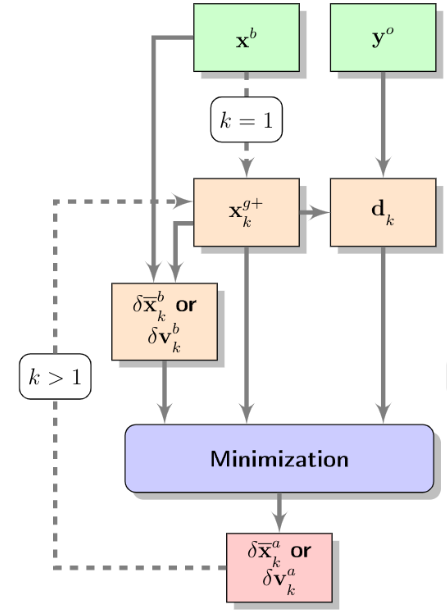
\includegraphics[width=0.3\linewidth]{fig/th.png}
  \caption{\label{fig01} Illustrative workflow of the theoretical method. The full resolution background and guess are used at each outer iteration to compute the $\delta \overline{\mathbf{x}}^b_k$ or $\delta \mathbf{v}^b_k$, using $\mathbf{B}_k^{-1}$:}
 \end{center}
\end{figure}

\begin{figure}[H]
 \begin{center}
  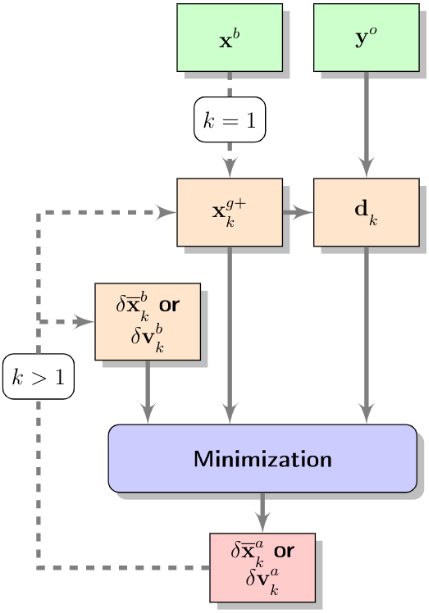
\includegraphics[width=0.3\linewidth]{fig/std.png}
  \caption{\label{fig02} Illustrative workflow of the standard method. The potential guess inconsistency of the "standard" method comes from the fork in the use of the minimization output, to compute the full resolution guess and the first term of the right-hand side independently. If the correct formula is not used, then a guess inconsistency can arise.}
 \end{center}
\end{figure}

\begin{figure}[H]
 \begin{center}
  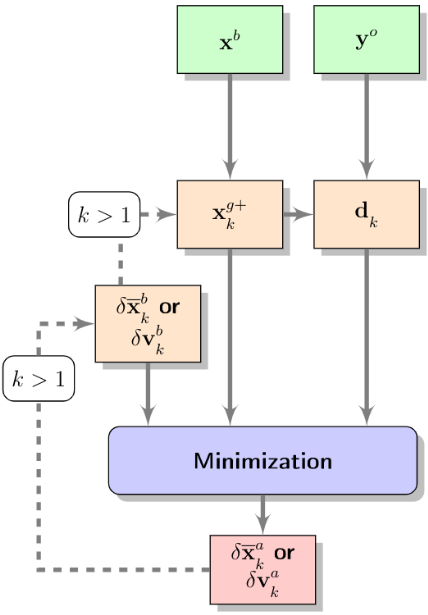
\includegraphics[width=0.3\linewidth]{fig/cst.png}
  \caption{\label{fig03} Illustrative workflow of the consistent method. Because of it closed cycle form (no fork), the "consistent" method ensures the guess consistency, without requiering $\mathbf{B}_k^{-1}$.}
 \end{center}
\end{figure}

The fork in the "standard" method using the analysis of iteration $k$ to compute separately the background increment and the guess of iteration $k+1$ is responsible of the potential inconsistency of the guess. 

The differences between the three methods coming from this guess inconsistency are illustraed using a toy problem which is describe in section \ref{sec:res}.

Another important problem is the equivalence between the square root $\mathbf{B}$ preconditionning and the full $\mathbf{B}$ preconditionning which may also be used for computationnal efficiency. This equivalence in the case of a multi-incremental multi-resolution framework is discussed in the following section.


\section{Equivalence between preconditionners}
(NB: or "full B precontionning" - is it necessary to put the equations ? Maybe we can just say that the same steps can be realized with B.)

Another preconding technique consists in defining a new variable $\delta \overline{\mathbf{x}}_k = \mathbf{B}_k^{-1} \delta \mathbf{x}_k$ so that the linear system to solve can be written as:
\begin{align}
 \mathbf{A}^{\overline{\mathbf{x}}}_k \delta \overline{\mathbf{x}}^a_k = \mathbf{b}^{\overline{\mathbf{x}}}_k,
\end{align}
 $\delta \overline{\mathbf{x}}^a_k$ being the preconditionned analysis increment, and with:
 \begin{align}
  \mathbf{A}^{\overline{\mathbf{x}}}_k = \mathbf{I}_n + \mathbf{H}_k^\mathrm{T} \mathbf{R}^{-1} \mathbf{H}_k \mathbf{B}_k,
 \end{align}
 and the right hand side now written as:
 \begin{align}
  \mathbf{b}^{\overline{\mathbf{x}}}_k =  \delta \overline{\mathbf{x}}^b_k + \mathbf{H}_k^\mathrm{T} \mathbf{R}^{-1} \mathbf{d}_k.
 \end{align}
 
An equivalent form of equation \eqref{eq:back_inc_B} can be found by applying $\mathbf{B}^{-1}$ on both side of equation \eqref{eq:back_inc} to express the so preconditionned background increment as:
\begin{align}
\label{eq:back_inc_B}
\delta \overline{\mathbf{x}}^b_k = - \sum_{i=1}^{k-1} \delta \overline{\mathbf{x}}^a_i.
\end{align}
In the same way as for the square root $\mathbf{B}$ preconditionning, if the $\mathbf{B}$ matrix changes between the outer loops and so depends on $k$, one can write:
\begin{align}
\label{eq:back_inc_B_diff}
\delta \overline{\mathbf{x}}^b_k & = - \mathbf{B}_k^{-1}\sum_{i=1}^{k-1} \delta \mathbf{x}^a_i \nonumber \\
& = - \sum_{i=1}^{k-1} \mathbf{B}_k^{-1} \mathbf{B}_i \delta \overline{\mathbf{x}}^a_i
\end{align}
and similarly if $\mathbf{B}_k^{-1} \mathbf{B}_i \delta \overline{\mathbf{x}}^a_i \ne \delta \overline{\mathbf{x}}^a_i$, equation \eqref{eq:back_inc_B} cannot be used consistently.

One can also write equivalent forms of equations \eqref{eq:back_inc_Uvar} and \eqref{eq:correct_dvb_2} using this preconditionner in the "standard" method:
\begin{align}
\label{eq:back_inc_Bvar}
\delta \overline{\mathbf{x}}^b_k = - \sum_{i=1}^{k-1} \mathbf{T}^\mathbf{x}_{i \rightarrow k} \delta \overline{\mathbf{x}}^a_i,
\end{align}
\begin{align}
\label{eq:correct_dxb_2}
\delta \overline{\mathbf{x}}^b_k & = -\mathbf{B}^{-1}_k \mathbf{T}^\mathbf{x}_{K \rightarrow k} \sum_{i=1}^{k-1} \delta \mathbf{x}^{a+}_i.
\end{align}
Now comparing equations \eqref{eq:back_inc_Bvar} and \eqref{eq:correct_dxb_2}, the guess consistency is maintained if:
\begin{align}
\label{eq:general_condition_B}
& \mathbf{B}^{-1}_k \mathbf{T}^\mathbf{x}_{K \rightarrow k} \sum_{i=1}^{k-1} \delta \mathbf{x}^{a+}_i = \sum_{i=1}^{k-1} \mathbf{T}^\mathbf{x}_{i \rightarrow k} \delta \overline{\mathbf{x}}^a_i, \nonumber \\
\Leftrightarrow \ & \mathbf{T}^\mathbf{x}_{K \rightarrow k} \sum_{i=1}^{k-1} \delta \mathbf{x}^{a+}_i = \mathbf{B}_k \sum_{i=1}^{k-1} \mathbf{T}^\mathbf{x}_{i \rightarrow k} \delta \overline{\mathbf{x}}^a_i, \nonumber \\
 \Leftrightarrow \ & \boxed{\mathbf{T}^\mathbf{x}_{K \rightarrow k} \delta \mathbf{x}^{a+}_{k-1} =  \mathbf{B}_k \sum_{i=1}^{k-1} \mathbf{T}^\mathbf{x}_{i \rightarrow k} \delta \overline{\mathbf{x}}^a_i - \mathbf{T}^\mathbf{x}_{K \rightarrow k} \sum_{i=1}^{k-2} \delta \mathbf{x}^{a+}_i}.
\end{align}
Once again, one can write a complete "expression" of the full resolution analysis increment if a right inverse exists for the interpolation operator:
%\begin{align}
%\label{eq:general_condition_B_K2}
%\delta \mathbf{x}^{a+}_1 =  \mathbf{B}_2 \mathbf{T}^\mathbf{x}_{1 \rightarrow 2} \delta \overline{\mathbf{x}}^a_1
%\end{align}
\begin{align}
\label{eq:general_condition_B_right_inverse}
\delta \mathbf{x}^{a+}_{k-1} =  \left(\mathbf{T}^\mathbf{x}_{K \rightarrow k}\right)^{-1}_\text{right} \left(\mathbf{B}_k \sum_{i=1}^{k-1} \mathbf{T}^\mathbf{x}_{i \rightarrow k} \delta \overline{\mathbf{x}}^a_i - \mathbf{T}^\mathbf{x}_{K \rightarrow k} \sum_{i=1}^{k-2} \delta \mathbf{x}^{a+}_i\right),
\end{align}
leading to:
\begin{align}
\label{eq:transitive_condition_B}
\delta \mathbf{x}^{a+}_{k-1} = \mathbf{T}^\mathbf{x}_{k \rightarrow K} \left(\mathbf{B}_k \sum_{i=1}^{k-1} \mathbf{T}^\mathbf{x}_{i \rightarrow k} \delta \overline{\mathbf{x}}^a_i - \mathbf{T}^\mathbf{x}_{K \rightarrow k} \sum_{i=1}^{k-2} \delta \mathbf{x}^{a+}_i\right),
\end{align}
in the case of transitive interpolators.
The right-hand side of equation \eqref{eq:transitive_condition_B} can be split to extract the term coming from outer iteration $k-1$:
\begin{align}
\delta \mathbf{x}^{a+}_{k-1} = \mathbf{T}^\mathbf{x}_{k \rightarrow K} \mathbf{B}_k \mathbf{T}^\mathbf{x}_{k-1 \rightarrow k} \delta \overline{\mathbf{x}}^a_{k-1} + \mathbf{T}^\mathbf{x}_{k \rightarrow K} \sum_{i=1}^{k-2} \left(\mathbf{B}_k \mathbf{T}^\mathbf{x}_{i \rightarrow k} \delta \overline{\mathbf{x}}^a_i - \mathbf{T}^\mathbf{x}_{K \rightarrow k} \delta \mathbf{x}^{a+}_i\right),
\end{align}
and if the $\mathbf{B}$ family is projective, then:
\begin{align}
\mathbf{T}^\mathbf{x}_{k \rightarrow K} \mathbf{B}_k \mathbf{T}^\mathbf{x}_{k-1 \rightarrow k} & = \mathbf{T}^\mathbf{x}_{k \rightarrow K} \mathbf{T}^\mathbf{x}_{k-1 \rightarrow k} \mathbf{B}_{k-1} \nonumber \\ 
& = \mathbf{T}^\mathbf{x}_{k-1 \rightarrow K} \mathbf{B}_{k-1}
\end{align}
so a simplified expression of $\delta \mathbf{x}^{a+}_{k-1}$ can be written as:
\begin{align}
\label{eq:projective_condition_B}
\boxed{\delta \mathbf{x}^{a+}_{k-1} = \mathbf{T}^\mathbf{x}_{k-1 \rightarrow K} \mathbf{B}_{k-1} \delta \overline{\mathbf{x}}^a_{k-1}}
\end{align}
that verifies \eqref{eq:transitive_condition_B} since both terms inside the summation cancel each other:
\begin{align}
\mathbf{B}_k \mathbf{T}^\mathbf{x}_{i \rightarrow k} \delta \overline{\mathbf{x}}^a_i - \mathbf{T}^\mathbf{x}_{K \rightarrow k} \delta \mathbf{x}^{a+}_i & = \mathbf{B}_k \mathbf{T}^\mathbf{x}_{i \rightarrow k} \delta \overline{\mathbf{x}}^a_i - \mathbf{T}^\mathbf{x}_{K \rightarrow k}  \mathbf{T}^\mathbf{x}_{i \rightarrow K} \mathbf{B}_i \delta \overline{\mathbf{x}}^a_i \nonumber \\
& = \left(\mathbf{B}_k \mathbf{T}^\mathbf{x}_{i \rightarrow k} - \mathbf{T}^\mathbf{x}_{i \rightarrow k} \mathbf{B}_i \right) \delta \overline{\mathbf{x}}^a_i \nonumber \\
& = 0
\end{align}

Finally, in the consistent methos, the background increment is simply obtained as:
\begin{align}
\label{eq:alternative_B}
\delta \mathbf{x}^b_k & = \mathbf{B}_k \delta \overline{\mathbf{x}}^b_k.
\end{align}

The full $\mathbf{B}$ preconditionning is mathematically equivalent to the square root $\mathbf{B}$ one, but in the case of a multi-incremental multi-resolution scheme where the $\mathbf{B}$ matrix depends on $k$, this equivalence is not guaranteed anymore. We discuss this point in more details in section \ref{sec:res}.


%---------------------------------------------------------------------------------
\section{Methodology and results}
\label{sec:res}
In order to illustrate the differences arising between the three methods due to the guess consistency, we have compared the results obtained with all the methods on a toy problem detailed in the present section.

\subsection{Methodology}
In this section we illustrate the differences arising between the three above-mentionned methods related to the guess consistency. To do so, we have built a bidimensional toy problem as follows:
\begin{itemize}
 \item We consider a periodic domain composed of bidimensional square grids with $m_x=101$ x-coordinates and $m_y=101$ y-coordinates (leading to a total of $m = m_x \times m_y$ points) and assume that this resolution corresponds to the full resolution of our prolem (e.g. this resolution corresponds to the last iteration $k=K$ of our multi-incremental multi-resolution scheme).
 \item A $\mathbf{B}$ matrix is introduced with gaussian spectral variances defined as:
 \begin{align}
  \mathbf{B_{k,l}} = e^{-2((k^2 + l^2)\pi L_b)^2}, 
 \end{align}
 where $k \in [0:m_x/2]$, $l \in [-m_y/2:m_y/2]$ are the accessible wave numbers and $L_b$ is a correlation lenghtscale.
 We also define its grid point variance as:
 (NB: quand on prend sigmabvar = 0, quest ce qu'on fait ?)
 \begin{align}
 \mathbf{B_{i,j}} = 1 + \sigma^b \sin(2\pi x_i) \sin(2\pi y_j),  
 \end{align}
where $\sigma^b$ can be modified, $x_i$ is the $i^{th}$ x-coordinate of the grid, and $y_j$ is the $j^{th}$ y-coordinate of the grid.
 \item A full resolution truth state $\mathbf{x^t}$ is defined on this grid by applying the square root of $\mathbf{B}$ (denoted $\mathbf{U}$) on a random field $\nu^{t}$ with normal distribution: (NB: I do not remember why is there $x^t = 1+x^t$ in the code? - Find a way to write the identity operator):
 \begin{align}
 \mathbf{x}^t = 1_m + \mathbf{U}\nu^{t}.
 \end{align}
 \item A full resolution background state is defined in same manner with a different random field $\nu^{b}$ (NB: idem for this):
 \begin{align}
 \mathbf{x}_b=\mathbf{x}^t + \mathbf{U}\nu^{b}.
 \end{align}
 \item In order to have the simpler problem, the observation operator is taken to be the identity. We also introduce $p=2000$ observation points that are not necessarily on grids points, and a linear observation operator: (NB: we do not discuss about the cubic version ?)
 \begin{align}
  \mathcal{H}\mathbf{x} = \mathbf{x}. 
 \end{align}
 \item Finally the observation error covariance matrix $\mathbf{R} \in \mathbb{R}^{p \times p}$ is simply defined as:
 \begin{align}
 \mathbf{R}_{i,j} = \sigma^o.
 \end{align}
\end{itemize}

In order to illustrate the differences between the different cases we have mentioned, we applied a multi-incremental multi-resolution scheme using the three methods as well as different interpolators. The spectral decomposition is an orthogonal operator, which can be associated with a zero padding operator to build a transitive interpolator. It should be noted that usual grid-points interpolators like (bi-)linear and nearest-neighbor interpolators are not transitive in general. An important exception is the (bi-)linear interpolator which is transitive when coarse grid points are colocated with fine grid points.

\subsection{Results}
NB:Show the quadratic cost function (obs and background) + tables + xgstd-xgth.

To illustrate the differences between the different cases that we have mentionned, we have choosen to use a spectral interpolation as a transitive interpolator, and we also have tested bilinear interpolation which is transitive if the grid points of different iterations are colocated. We arbitrarily have taken the values of $L_b = 0.1$, $\sigma^o=0.1$. According to the convergence of our algorithm, we decided to realize 6 outer loops of 3 inner loops. The change of resolution is as follows:$\mathcal{R}_1 = $, $\mathcal{R}_2 = $ ...

As expected, in the first case where transitive a interpolator is used, with a projective $\mathbf{B}$ matrix family, all the methods give the same results, and the two preconditionners are equivalent at machine precision.

The fact that the cost function shows small peaks at each beginning of outer loop is due to the relinearization of the problem around the new guess as well as the change of resolution, making the problem different from the one that have been solved at the previous outer loop.

The tables (\ref{tab:}) to (\ref{tab:}) summerize the differences or equivalence between the three methods and the two preconditionners in the case of a transitive interpolator and a "projective" $\mathbf{B}$ matrix family (), 





%---------------------------------------------------------------------------------


\conclusions  %% \conclusions[modified heading if necessary]
Multi-incremental multi-resolution scheme is a powerfull way to improve computational efficiency of DA problems solving and might be more and more used in operational DA systems in a near future. In such an approach, we have shown that the question of the guess consistency is crucial since the results can be very different from a method to another according to the way the guess is calculated. We have discussed in detail this question and have shown that the choice of the interpolation operator used to realize the change of resolution at the outer loop level was very important. We have defined a class of interpolators called "transitive" interpolators that satisfy certain conditions ensuring the guess consistency. A subcase of transitive interpolators have been discussed concerning the $\mathbf{B}$ matrix family, introducing the "projective" $\mathbf{B}$ matrices for which low resolution members can be obtained from the high resolution ones using transitive interpolators. In this case, a simplified expression can be derived for the analysis increment and only the previous iteration is needed instead of all the previous ones.

Through a toy DA problem, we have illustrated that in the "standard" method currently used in operational DA systems, the way the guess is used in the minimization is inconsistent and could give results that are very different from the theoretical ones. We introduced a new "consistent" method to compute the guess based on the idea of reversing the order of calculations. This method have two strong advantages: first, it ensures the guess consistency, and second, it requires much more simpler calculations. We have shown the ability of this method to reproduce the results of the "standard" one in the case where ().

We have also discussed the equivalence of two well known preconditionners in a multi-incremental multi-resolution context and have shown that this equivalence does not necessarily hold. It is maintained if transitive interpolators are used and the $\mathbf{B}$ matrix family is "projective". If these conditions are not satisfied, the differences in the cost functions obtained with the two preconditionners can be huge and grow with the outer iterations. 

%% The following commands are for the statements about the availability of data sets and/or software code corresponding to the manuscript.
%% It is strongly recommended to make use of these sections in case data sets and/or software code have been part of your research the article is based on.

%\codeavailability{TEXT} %% use this section when having only software code available


%\dataavailability{TEXT} %% use this section when having only data sets available


%\codedataavailability{TEXT} %% use this section when having data sets and software code available


%\sampleavailability{TEXT} %% use this section when having geoscientific samples available


%\videosupplement{TEXT} %% use this section when having video supplements available


\appendix



\noappendix       %% use this to mark the end of the appendix section. Otherwise the figures might be numbered incorrectly (e.g. 10 instead of 1).

%% Regarding figures and tables in appendices, the following two options are possible depending on your general handling of figures and tables in the manuscript environment:

%% Option 1: If you sorted all figures and tables into the sections of the text, please also sort the appendix figures and appendix tables into the respective appendix sections.
%% They will be correctly named automatically.

%% Option 2: If you put all figures after the reference list, please insert appendix tables and figures after the normal tables and figures.
%% To rename them correctly to A1, A2, etc., please add the following commands in front of them:

\appendixfigures  %% needs to be added in front of appendix figures

\appendixtables   %% needs to be added in front of appendix tables

%% Please add \clearpage between each table and/or figure. Further guidelines on figures and tables can be found below.



%\authorcontribution{TEXT} %% this section is mandatory

%\competinginterests{TEXT} %% this section is mandatory even if you declare that no competing interests are present

%\disclaimer{TEXT} %% optional section

%\begin{acknowledgements}
%TEXT
%\end{acknowledgements}




%% REFERENCES

%% The reference list is compiled as follows:

\begin{thebibliography}{}

\bibitem[AUTHOR(YEAR)]{LABEL1}
REFERENCE 1

\bibitem[AUTHOR(YEAR)]{LABEL2}
REFERENCE 2

\end{thebibliography}

%% Since the Copernicus LaTeX package includes the BibTeX style file copernicus.bst,
%% authors experienced with BibTeX only have to include the following two lines:
%%
%% \bibliographystyle{copernicus}
%% \bibliography{example.bib}
%%
%% URLs and DOIs can be entered in your BibTeX file as:
%%
%% URL = {http://www.xyz.org/~jones/idx_g.htm}
%% DOI = {10.5194/xyz}


%% LITERATURE CITATIONS
%%
%% command                        & example result
%% \citet{jones90}|               & Jones et al. (1990)
%% \citep{jones90}|               & (Jones et al., 1990)
%% \citep{jones90,jones93}|       & (Jones et al., 1990, 1993)
%% \citep[p.~32]{jones90}|        & (Jones et al., 1990, p.~32)
%% \citep[e.g.,][]{jones90}|      & (e.g., Jones et al., 1990)
%% \citep[e.g.,][p.~32]{jones90}| & (e.g., Jones et al., 1990, p.~32)
%% \citeauthor{jones90}|          & Jones et al.
%% \citeyear{jones90}|            & 1990



%% FIGURES

%% When figures and tables are placed at the end of the MS (article in one-column style), please add \clearpage
%% between bibliography and first table and/or figure as well as between each table and/or figure.

% The figure files should be labelled correctly with Arabic numerals (e.g. fig01.jpg, fig02.png).


%% ONE-COLUMN FIGURES

%%f
%\begin{figure}[t]
%\includegraphics[width=8.3cm]{FILE NAME}
%\caption{TEXT}
%\end{figure}
%
%%% TWO-COLUMN FIGURES
%
%%f
%\begin{figure*}[t]
%\includegraphics[width=12cm]{FILE NAME}
%\caption{TEXT}
%\end{figure*}
%
%
%%% TABLES
%%%
%%% The different columns must be seperated with a & command and should
%%% end with \\ to identify the column brake.
%
%%% ONE-COLUMN TABLE
%
%%t
%\begin{table}[t]
%\caption{TEXT}
%\begin{tabular}{column = lcr}
%\tophline
%
%\middlehline
%
%\bottomhline
%\end{tabular}
%\belowtable{} % Table Footnotes
%\end{table}
%
%%% TWO-COLUMN TABLE
%
%%t
%\begin{table*}[t]
%\caption{TEXT}
%\begin{tabular}{column = lcr}
%\tophline
%
%\middlehline
%
%\bottomhline
%\end{tabular}
%\belowtable{} % Table Footnotes
%\end{table*}
%
%%% LANDSCAPE TABLE
%
%%t
%\begin{sidewaystable*}[t]
%\caption{TEXT}
%\begin{tabular}{column = lcr}
%\tophline
%
%\middlehline
%
%\bottomhline
%\end{tabular}
%\belowtable{} % Table Footnotes
%\end{sidewaystable*}
%
%
%%% MATHEMATICAL EXPRESSIONS
%
%%% All papers typeset by Copernicus Publications follow the math typesetting regulations
%%% given by the IUPAC Green Book (IUPAC: Quantities, Units and Symbols in Physical Chemistry,
%%% 2nd Edn., Blackwell Science, available at: http://old.iupac.org/publications/books/gbook/green_book_2ed.pdf, 1993).
%%%
%%% Physical quantities/variables are typeset in italic font (t for time, T for Temperature)
%%% Indices which are not defined are typeset in italic font (x, y, z, a, b, c)
%%% Items/objects which are defined are typeset in roman font (Car A, Car B)
%%% Descriptions/specifications which are defined by itself are typeset in roman font (abs, rel, ref, tot, net, ice)
%%% Abbreviations from 2 letters are typeset in roman font (RH, LAI)
%%% Vectors are identified in bold italic font using \vec{x}
%%% Matrices are identified in bold roman font
%%% Multiplication signs are typeset using the LaTeX commands \times (for vector products, grids, and exponential notations) or \cdot
%%% The character * should not be applied as mutliplication sign
%
%
%%% EQUATIONS
%
%%% Single-row equation
%
%\begin{equation}
%
%\end{equation}
%
%%% Multiline equation
%
%\begin{align}
%& 3 + 5 = 8\\
%& 3 + 5 = 8\\
%& 3 + 5 = 8
%\end{align}
%
%
%%% MATRICES
%
%\begin{matrix}
%x & y & z\\
%x & y & z\\
%x & y & z\\
%\end{matrix}
%
%
%%% ALGORITHM
%
%\begin{algorithm}
%\caption{...}
%\label{a1}
%\begin{algorithmic}
%...
%\end{algorithmic}
%\end{algorithm}
%
%
%%% CHEMICAL FORMULAS AND REACTIONS
%
%%% For formulas embedded in the text, please use \chem{}
%
%%% The reaction environment creates labels including the letter R, i.e. (R1), (R2), etc.
%
%\begin{reaction}
%%% \rightarrow should be used for normal (one-way) chemical reactions
%%% \rightleftharpoons should be used for equilibria
%%% \leftrightarrow should be used for resonance structures
%\end{reaction}
%
%
%%% PHYSICAL UNITS
%%%
%%% Please use \unit{} and apply the exponential notation


\end{document}
